\documentclass{article}

% DK tikz stuff
\usepackage{placeins}
\usepackage{tikz}
\usepackage{tikzscale}
\usetikzlibrary{arrows}

\begin{document}

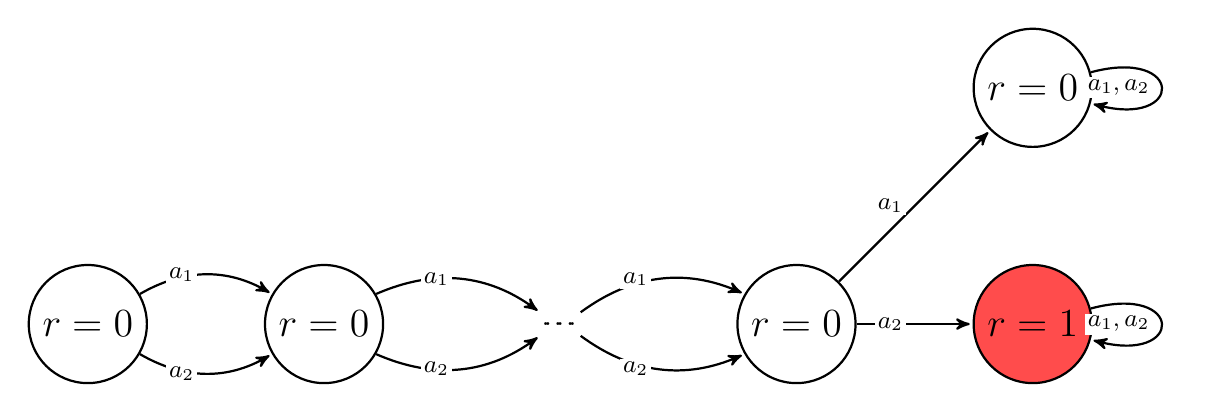
\begin{tikzpicture}
%\usetikzlibrary{calc}
  [->,>=stealth',shorten >=1pt,auto,node distance=3cm,
  thick,
	main node/.style={circle,fill=black!0,draw,
  font=\sffamily\Large\bfseries,minimum size=15mm},
	goal node/.style={circle,fill=red!70,draw,
  font=\sffamily\Large\bfseries,minimum size=15mm}]

  \node[goal node] (R) {$r=1$};
  \node[main node] (L) [above of=R] {$r=0$};
  \node[main node] (s3) [left of=R] {$r=0$};
  \node[draw=none] (s2) [left of=s3] {$\ldots$};
  \node[main node] (s1) [left of=s2] {$r=0$};
  \node[main node] (s0) [left of=s1] {$r=0$};

  \path[every node/.style={font=\sffamily\small,
  		fill=white,inner sep=1pt}]
    (s0) edge [bend right=30] node[left=1mm] {$a_2$} (s1)
        edge [bend left=30] node[left=1mm] {$a_1$} (s1)
    (s1) edge [bend right=30] node[left=1mm] {$a_2$} (s2)
        edge [bend left=30] node[left=1mm] {$a_1$} (s2)
    (s2) edge [bend right=30] node[left=1mm] {$a_2$} (s3)
        edge [bend left=30] node[left=1mm] {$a_1$} (s3)
	(s3) edge [bend right=0] node[left=1mm] {$a_2$} (R)
        edge [bend left=0] node[left=1mm] {$a_1$} (L)
    (R) edge [loop right] node[left=1mm] {$a_1, a_2$} (R)
    (L) edge [loop right] node[left=1mm] {$a_1, a_2$} (L);
    \path (s1) -- node[auto=false]{\ldots} (s3);
    %\node at ($(1)!.5!(2)$) {\ldots};
\end{tikzpicture}

\end{document}
